%%%%%%%%%%%%%%%%%%%%%%%%%%%%%%%%%%%%%%%%%%%%%%%%
%% Intro to LaTeX and Template for Homework Assignments
%% Quantitative Methods in Political Science
%% University of Mannheim
%% Fall 2018
%%%%%%%%%%%%%%%%%%%%%%%%%%%%%%%%%%%%%%%%%%%%%%%%

% created by Marcel Neunhoeffer & Sebastian Sternberg


% This template and tutorial will help you to write up your homework. It will also help you to use Latex for other assignments than this course's homework.

%%%%%%%%%%%%%%%%%%%%%%%%%%%%%%%%%%%%%%%%%%%%%%%%
% Before we get started
%%%%%%%%%%%%%%%%%%%%%%%%%%%%%%%%%%%%%%%%%%%%%%%%

% Make an account on overleaf.com and get started. No need to install anything.

%%%%%%%%%%%%%%%%%%%%%%%%%%%%%%%%%%%%%%%%%%%%%%%%
% Or if you want it the nerdy way...
% INSTALL LATEX: Before we can get started you need to install LaTeX on your computer.
				% Windows: http://miktex.org/download
				% Mac:         http://www.tug.org/mactex/mactex-download.html	
				% There a many more different LaTeX editors out there for both operating systems. I use TeXworks because it looks the same on Windows and Mac.
				

% SAVE THE FILE: The first thing you need to do is to save your LaTeX file in a directory as a .tex file. You will not be able to do anything else unless your file is saved. I suggest to save the .tex file in the same folder with your .R script and where you will save your plots from R to. Let's call this file template_homework1.tex and save it in your Week 1 folder.


% COMPILE THE FILE: After setting up your file, using your LaTeX editor (texmaker, texshop), you can compile your document using PDFLaTeX.
	% Compiling your file tells LaTeX to take the code you have written and create a pdf file
	% After compiling your file, in your directory will appear four new files, including a .pdf file. This is your output document.
	% It is good to compile your file regularly so that you can see how your code is translating into your document.
	
	
% ERRORS: If you get an error message, something is wrong in your code. Fix errors before they pile up!
	% As with error messages in R, google the exact error message if you have a question!
%%%%%%%%%%%%%%%%%%%%%%%%%%%%%%%%%%%%%%%%%%%%%%%%


% Now again for everyone...

% COMMANDS: 
	% To do anything in LaTeX, you must use commands
	% Commands tell LaTeX when to start your document, how you want your document to look, and how to format your document
	% Commands ALWAYS begin with a backslash \

% Everything following the % sign is a comment and will not be used by Latex to compile your document.
% This is very similar to # comments in R.

% Every .tex file usually consists of four parts.
% 1. Document Class
% 2. Packages
% 3. Header
% 4. Your Document

%%%%%%%%%%%%%%%%%%%%%%%%%%%%%%%%%%%%%%%%%%%%%%%%
% 1. Document Class
%%%%%%%%%%%%%%%%%%%%%%%%%%%%%%%%%%%%%%%%%%%%%%%%
 
 % The first command you will always have will declare your document class. This tells LaTeX what type of document you are creating (article, presentation, poster, etc). 
% \documentclass is the command
% in {} you specify the type of document
% in [] you define additional parameters
 
\documentclass[a4paper,12pt]{article} % This defines the style of your paper

% We usually use the article type. The additional parameters are the format of the paper you want to print it on and the standard font size. For us this is a4paper and 12pt.

%%%%%%%%%%%%%%%%%%%%%%%%%%%%%%%%%%%%%%%%%%%%%%%%
% 2. Packages
%%%%%%%%%%%%%%%%%%%%%%%%%%%%%%%%%%%%%%%%%%%%%%%%

% Packages are libraries of commands that LaTeX can call when compiling the document. With the specialized commands you can customize the formatting of your document.
% If the packages we call are not installed yet, TeXworks will ask you to install the necessary packages while compiling.

% First, we usually want to set the margins of our document. For this we use the package geometry. We call the package with the \usepackage command. The package goes in the {}, the parameters again go into the [].
\usepackage[top = 2.5cm, bottom = 2.5cm, left = 2.5cm, right = 2.5cm]{geometry} 

% Unfortunately, LaTeX has a hard time interpreting German Umlaute. The following two lines and packages should help. If it doesn't work for you please let me know.
\usepackage[T1]{fontenc}
\usepackage[utf8]{inputenc}

% The following two packages - multirow and booktabs - are needed to create nice looking tables.
\usepackage{multirow} % Multirow is for tables with multiple rows within one cell.
\usepackage{booktabs} % For even nicer tables.

% As we usually want to include some plots (.pdf files) we need a package for that.
\usepackage{graphicx} 

% The default setting of LaTeX is to indent new paragraphs. This is useful for articles. But not really nice for homework problem sets. The following command sets the indent to 0.
\usepackage{setspace}
\setlength{\parindent}{0in}

% Package to place figures where you want them.
\usepackage{float}

% The fancyhdr package let's us create nice headers.
\usepackage{fancyhdr}


%%%%%%%%%%%%%%%%%%%%%%%%%%%%%%%%%%%%%%%%%%%%%%%%
% 3. Header (and Footer)
%%%%%%%%%%%%%%%%%%%%%%%%%%%%%%%%%%%%%%%%%%%%%%%%

% To make our document nice we want a header and number the pages in the footer.

\pagestyle{fancy} % With this command we can customize the header style.

\fancyhf{} % This makes sure we do not have other information in our header or footer.

\lhead{\footnotesize GEO1001: Homework 1}% \lhead puts text in the top left corner. \footnotesize sets our font to a smaller size.

%\rhead works just like \lhead (you can also use \chead)
\rhead{\footnotesize Name (Konstantinos Pantelios)} %<---- Fill in your lastnames.

% Similar commands work for the footer (\lfoot, \cfoot and \rfoot).
% We want to put our page number in the center.
\cfoot{\footnotesize \thepage} 


%%%%%%%%%%%%%%%%%%%%%%%%%%%%%%%%%%%%%%%%%%%%%%%%
% 4. Your document
%%%%%%%%%%%%%%%%%%%%%%%%%%%%%%%%%%%%%%%%%%%%%%%%

% Now, you need to tell LaTeX where your document starts. We do this with the \begin{document} command.
% Like brackets every \begin{} command needs a corresponding \end{} command. We come back to this later.

\begin{document}


%%%%%%%%%%%%%%%%%%%%%%%%%%%%%%%%%%%%%%%%%%%%%%%%
%%%%%%%%%%%%%%%%%%%%%%%%%%%%%%%%%%%%%%%%%%%%%%%%

%%%%%%%%%%%%%%%%%%%%%%%%%%%%%%%%%%%%%%%%%%%%%%%%
% Title section of the document
%%%%%%%%%%%%%%%%%%%%%%%%%%%%%%%%%%%%%%%%%%%%%%%%

% For the title section we want to reproduce the title section of the Problem Set and add your names.

\thispagestyle{empty} % This command disables the header on the first page. 

\begin{tabular}{p{15.5cm}} % This is a simple tabular environment to align your text nicely 
{\large \bf Sensing Technologies and Mathematics for Geomatics} \\
GEO1001.2020 \\ MSc Geomatics \\ Delft University of Technology \\
\hline % \hline produces horizontal lines.
\\
\end{tabular} % Our tabular environment ends here.

\vspace*{0.3cm} % Now we want to add some vertical space in between the line and our title.

\begin{center} % Everything within the center environment is centered.
	{\Large \bf Homework 1} % <---- Don't forget to put in the right number
	\vspace{2mm}
	
        % YOUR NAMES GO HERE
	{\bf Name Konstantinos Pantelios, (5374367)} % <---- Fill in your names here!
		
\end{center}  

\vspace{0.4cm}

%%%%%%%%%%%%%%%%%%%%%%%%%%%%%%%%%%%%%%%%%%%%%%%%
%%%%%%%%%%%%%%%%%%%%%%%%%%%%%%%%%%%%%%%%%%%%%%%%

% Up until this point you only have to make minor changes for every week (Number of the homework). Your write up essentially starts here.
The data that were used in the following report were extracted from TU Dleft data portal. \cite{Maiullari2020}


\section{\it After lesson A1:}
\subsection{\it Compute mean statistics (mean, variance and standard deviation for each of the sensors variables), what do you observe from the results?} % <--- For future Homework sets you of course have to change the questions.




For 1.1, the code computes the mean, 
the variance and the standard deviation of 
all the different variables (19) from sensors A, B, C, D and E. 
The results (Figure 1) are displayed separately for each of the sensors and each variable takes occupies different rows.




\begin{figure}[H]
    \centering
    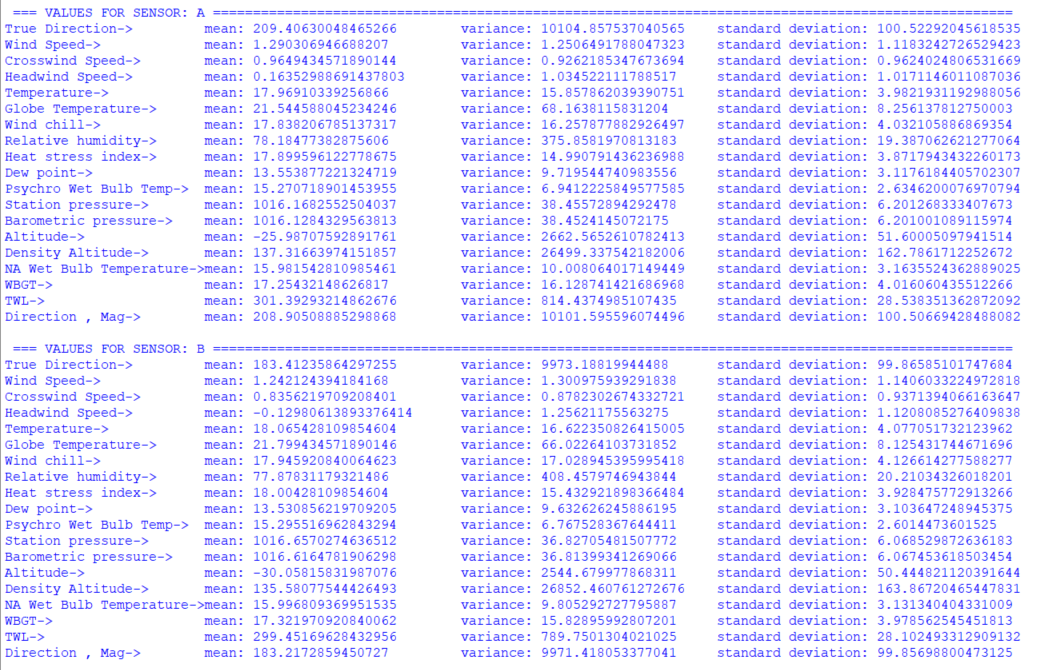
\includegraphics[width=\textwidth]{Graphs/Statistcal Indicators AB.PNG}
\end{figure}
\begin{figure}[H]
\centering
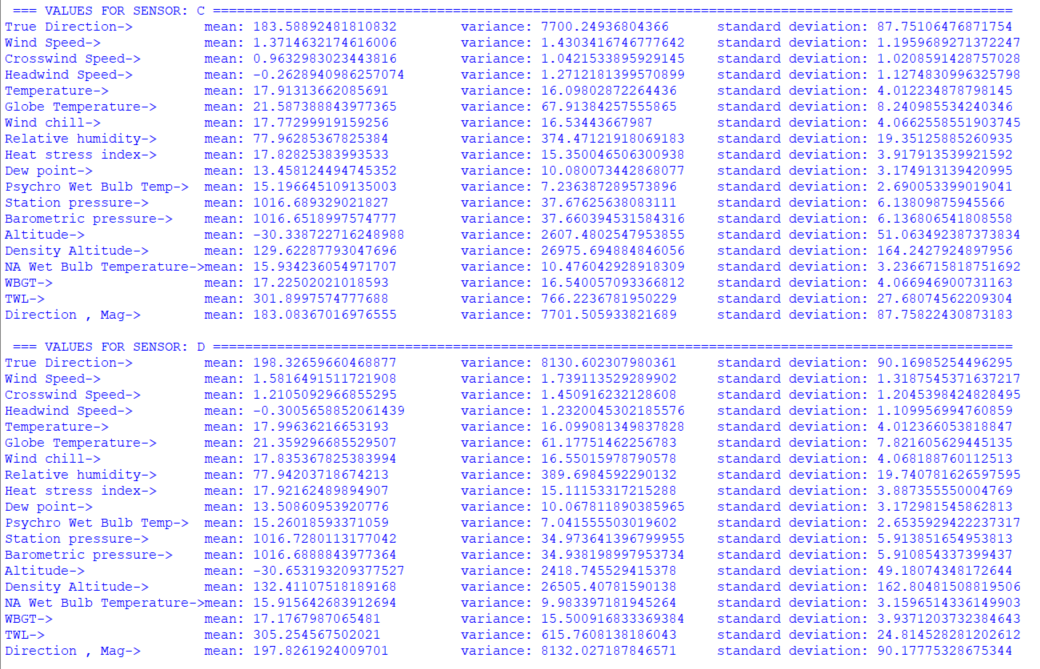
\includegraphics[width=\textwidth]{Graphs/Statistcal Indicators CD.PNG}
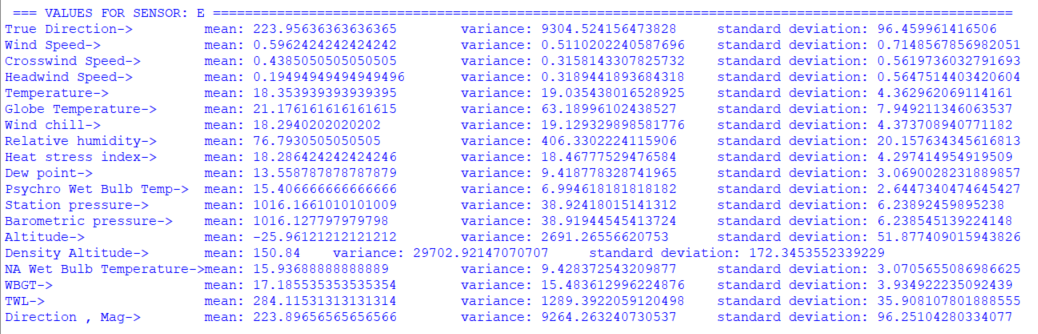
\includegraphics[width=\textwidth]{Graphs/Statistcal Indicators E.PNG}
\caption{\it'Mean, variance and standard deviation for each variable of the 5 sensors'}
\end{figure}




From a first glance we can see that in most variables the statistical indicators hold similar values between all the sensors.




There is a notable observation that can be derived from the variables Altitude and Density Altitude. 
The difference between mean and the standard deviations is such that could be only possible if the sensors are NOT fixated on the ground. 
So, we can hypothesize that all the sensors are strapped on balloons or drones and the measurement are taken from different heights
Looking at the variable Wind Direction, True, it is apparent that the wind was rarely blowing from the North (in comparison to the other directions),
which is information that can be used to calculate various correlations.




In general, there many different but related variables and the statistical indicators can reveal, 
on a surface level, possible correlations and interesting underlying facts or questions.




\subsection{\it Create 1 plot that contains histograms for the 5 sensors Temperature values. Compare histograms with 5 and 50 bins, why is the number of bins important?}




For 1.2, the codes computes and plots the Temperature
histograms of 5 and 50 bins for each of the 5 different sensors. 
The following figure (Figure 2) illustrates the above comment in 10 different 
plots where each row of plots corresponds to each sensor and each column 
correspond to the histogram with the respective number of bins.



\begin{figure}[H]
\centering
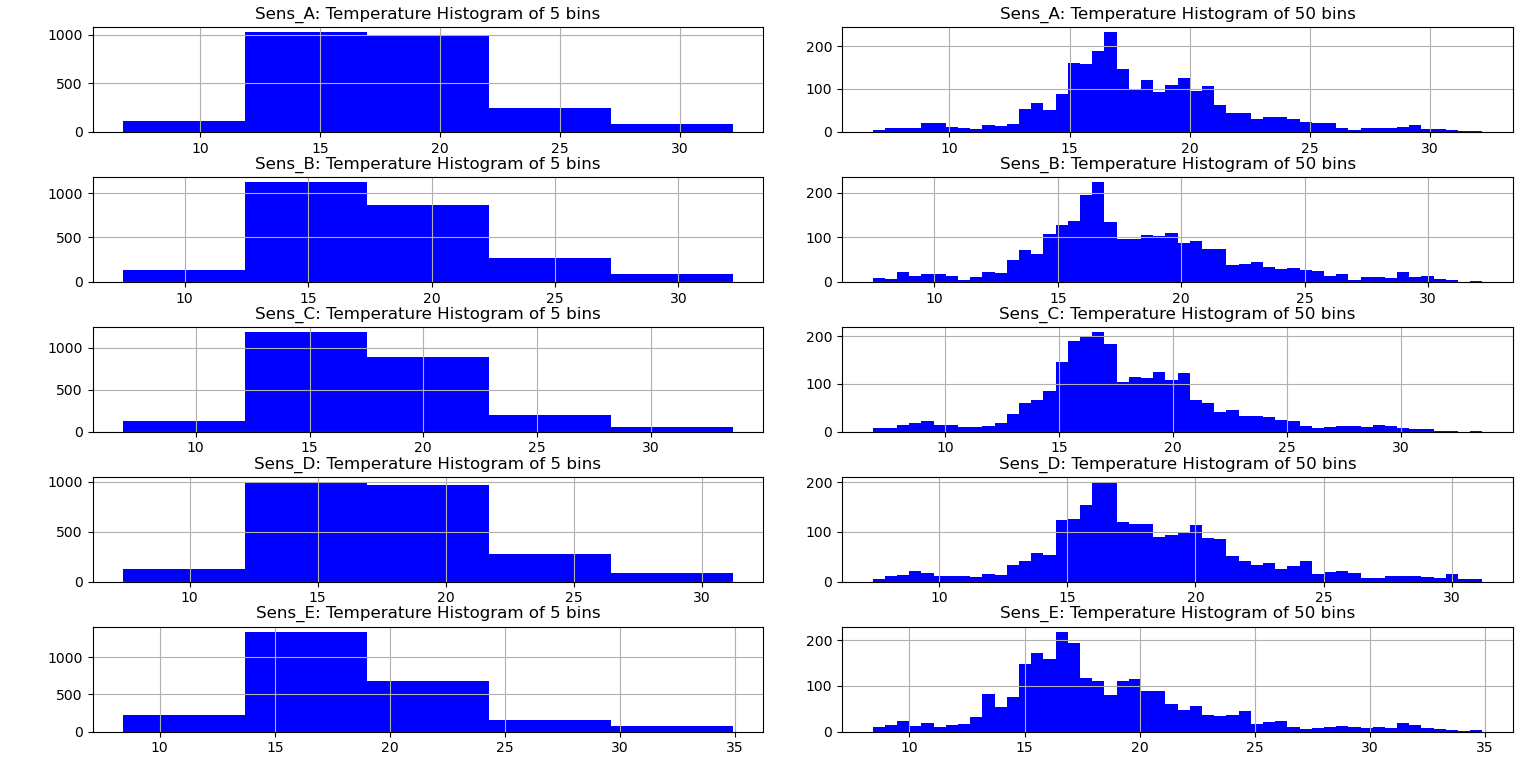
\includegraphics[width=\textwidth]{Graphs/Bin_comparison_of_5_sensor_Temperature_Histogram.png}
\caption{\it'Bin comparison of 5 sensor Temperature Histogram'}
\end{figure}




It is immediately apparent that the number of bins in a histogram plays a 
major role in the transmission of the message that plot tries to convey. 
Basically, the number of bins depend on the scale of data (values) 
that need to be illustrated. As such, five (5) bins are not enough 
to be able to get substantial information from almost 2.500 different 
values and we lose important levels of detail. On the other hand, using 
50 bins allows the graph to show much more detailed results. However, too 
many bars can also hinder the overall illustration of the figure.




Having that in mind I continue to code and plot the rest of the graphs using 30 bins when needed.  




\subsection{\it Create 1 plot where frequency poligons for the 5 sensors Temperature values overlap in different colours with a legend.}




For 1.3, the code generates a plot of the frequency polygons for 
the variable Temperature, for each of the 5 sensors. 
The frequency polygons graph (Figure 3) derives from a Temperature CDF 
stepped histogram of 50 bins and the 5 sensors are overlapping each other with 
different colours.



\begin{figure}[H]
\centering
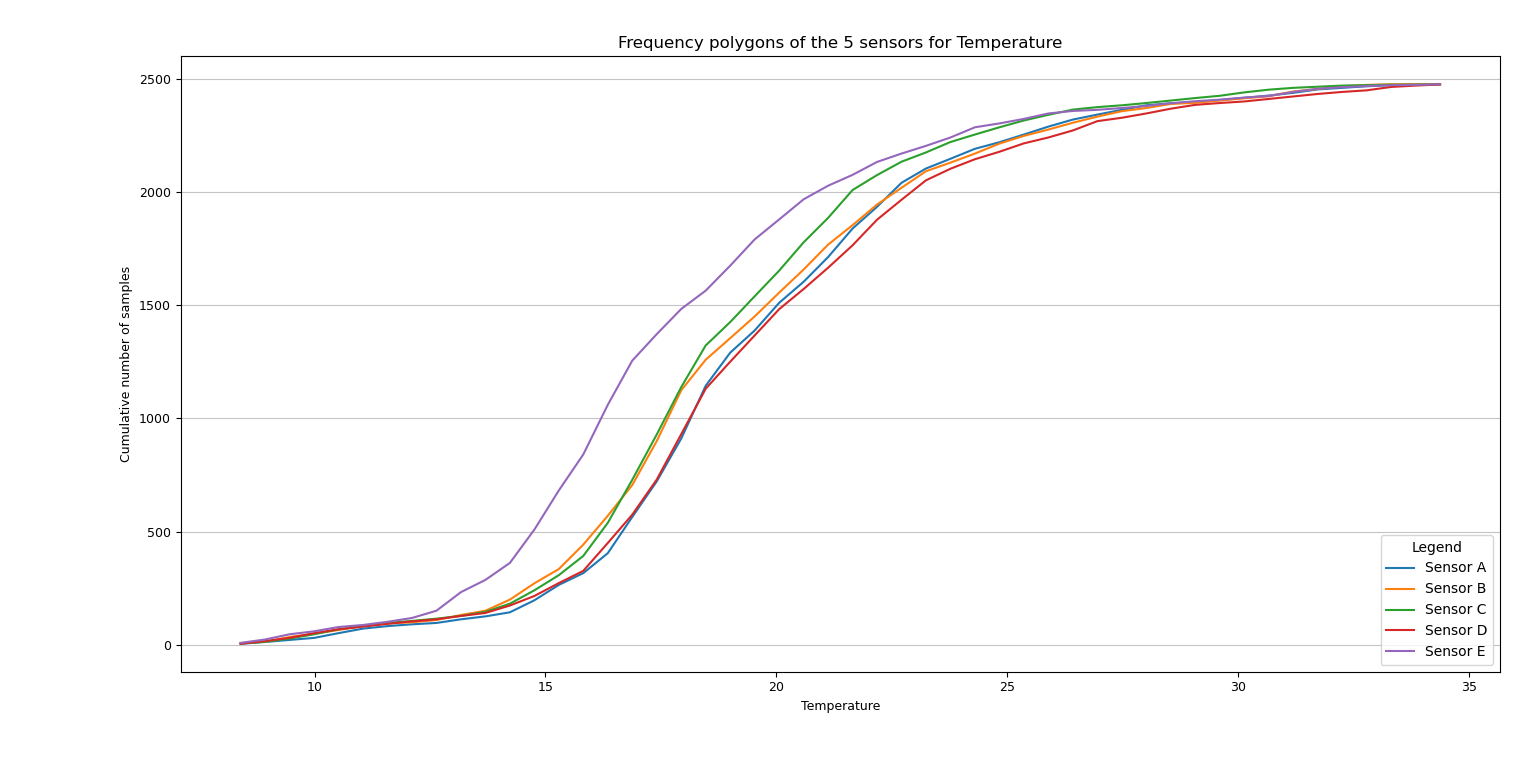
\includegraphics[width=\textwidth]{Graphs/Frequency_polygons_of_Temperature.png}
\caption{\it'Frequency polygons of the 5 sensors for Temperature'}
\end{figure}



\subsection{\it Generate 3 plots that include the 5 sensors boxplot for: Wind Speed, Wind Direction and Temperature.}




For 1.4, the code creates box-plots for the 
variables Wind Speed, Wind Direction and Temperature. 
The figure (Figure 4) shows the 3 different plots side by side 
with their respective variables’ values for the x axis and the 5 
different sensors as the boxes. The plot provides visualization 
of min, max, 25th, 50th,75th percentiles, mean and outliers.




\begin{figure}[H]
\centering
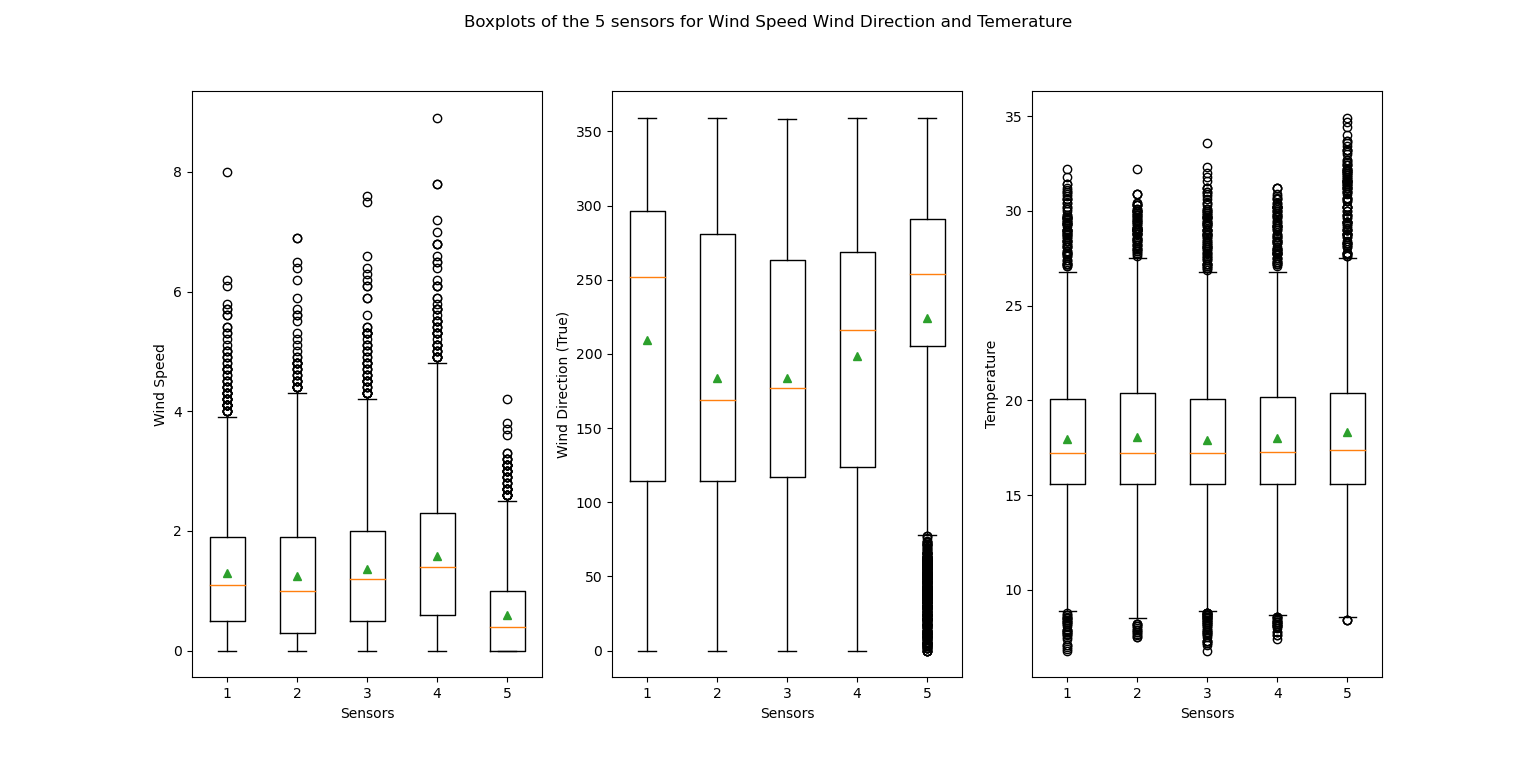
\includegraphics[width=\textwidth]{Graphs/Boxplots_of_the_5_sensors_for_Temerature,_Wind_Speed_and_Wind_Direction.png}
\caption{\it'Boxplots of the 5 sensors for Wind Speed Wind Direction and Temerature'}
\end{figure}




\section{\it After lesson A2:}
\subsection{\it Plot PMF, PDF and CDF for the 5 sensors Temperature values in independent plots (or subplots). Describe the behaviour of the distributions, are they all similar? what about their tails?}



For 2.1, the code computes and plots the PMF, PDF and 
CDF for the variable Temperature and for each of the 5 sensors. 
The figures (Figure 5, Figure 6, Figure 7) illustrate the above by combining the 5 sensors
in one figure every time in order to display the 3 distributions separately.



\begin{figure}[H]
\centering
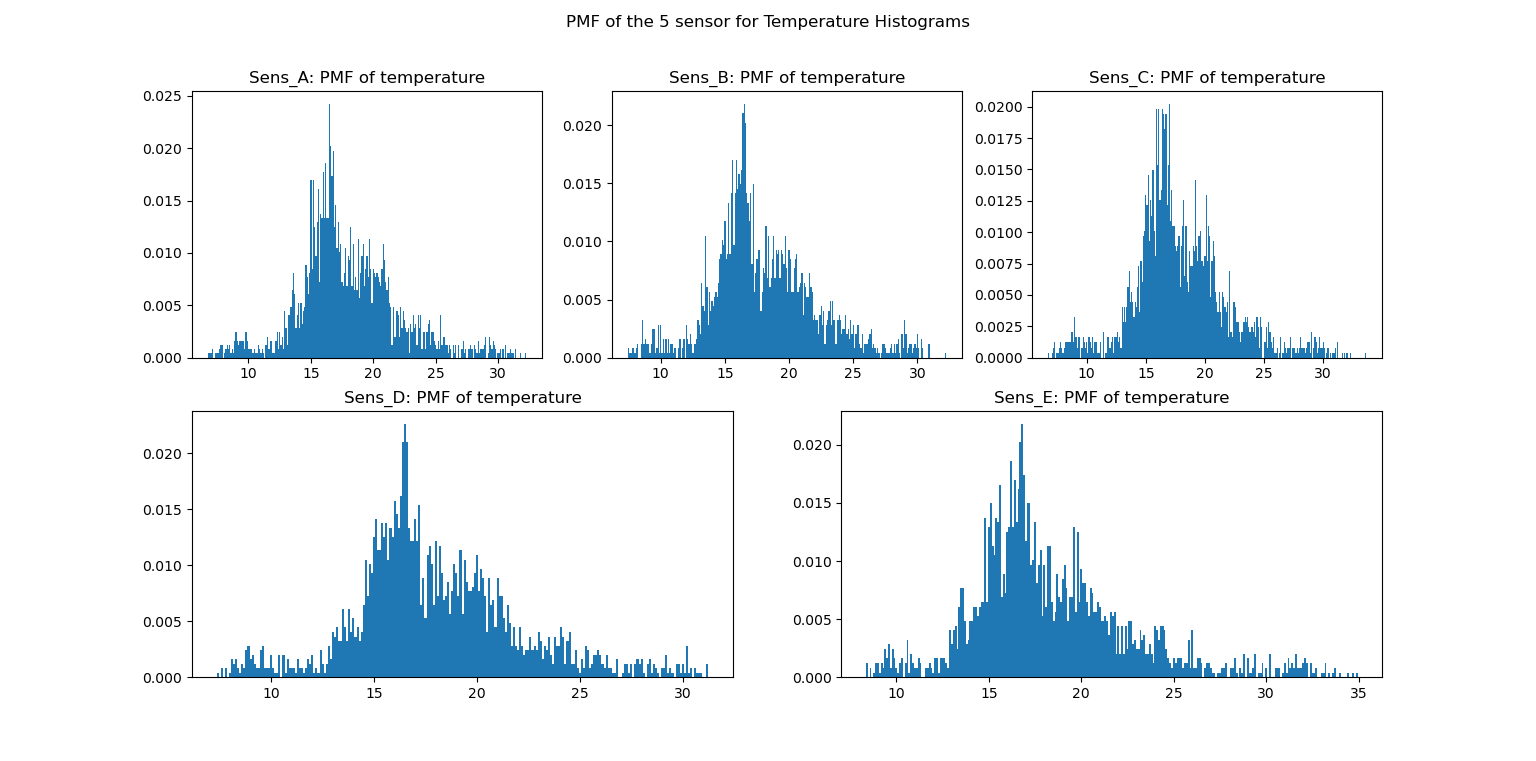
\includegraphics[width=\textwidth]{Graphs/PMF_of_the_5_sensor_-_Temperature_Histogram.png}
\caption{\it'PMF of the 5 sensor for Temperature Histograms'}
\end{figure}




\begin{figure}[H]
\centering
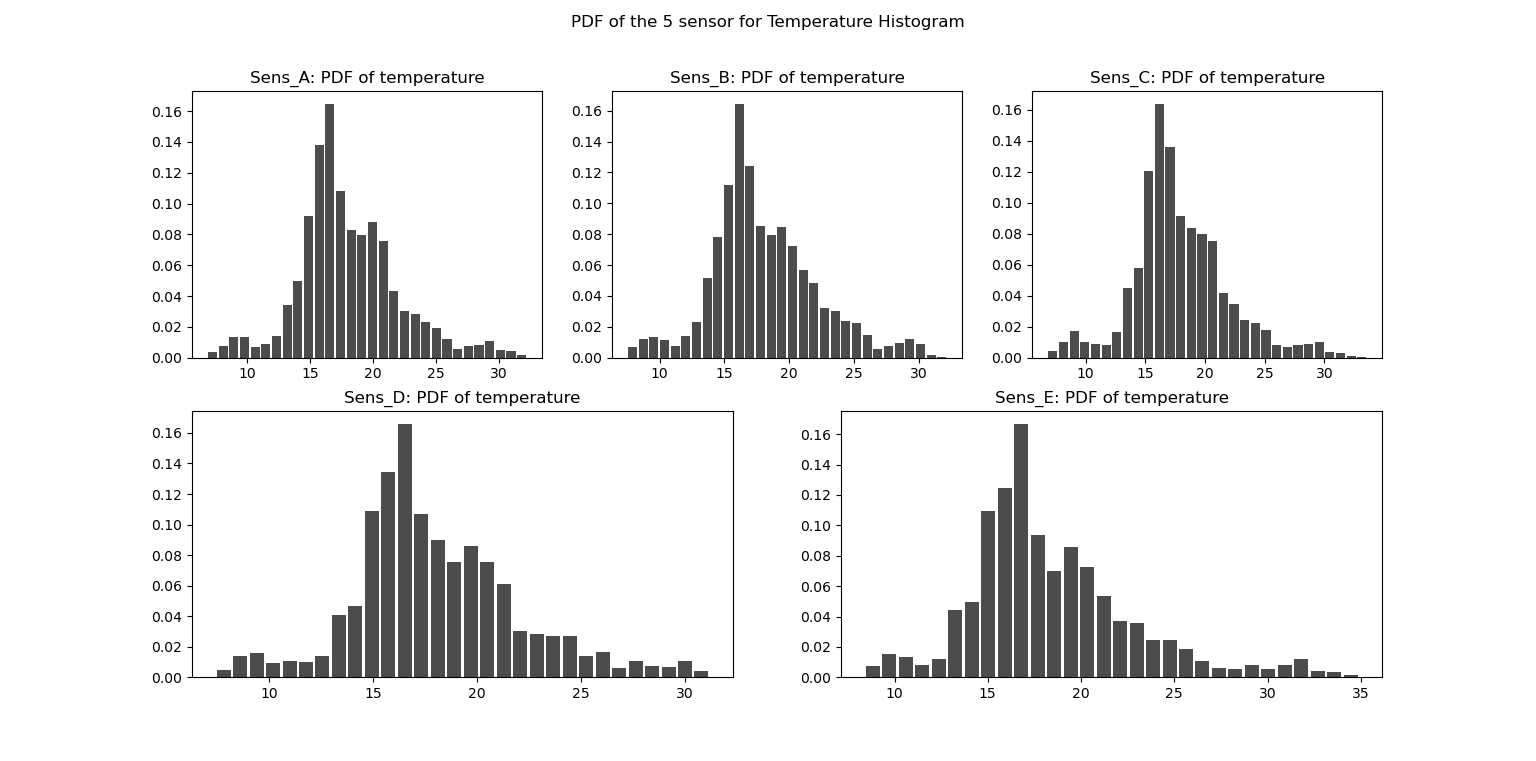
\includegraphics[width=\textwidth]{Graphs/PDF_of_the_5_sensor_-_Temperature_Histogram.png}
\caption{\it'PDF of the 5 sensor for Temperature Histograms'}
\end{figure}




\begin{figure}[H]
\centering
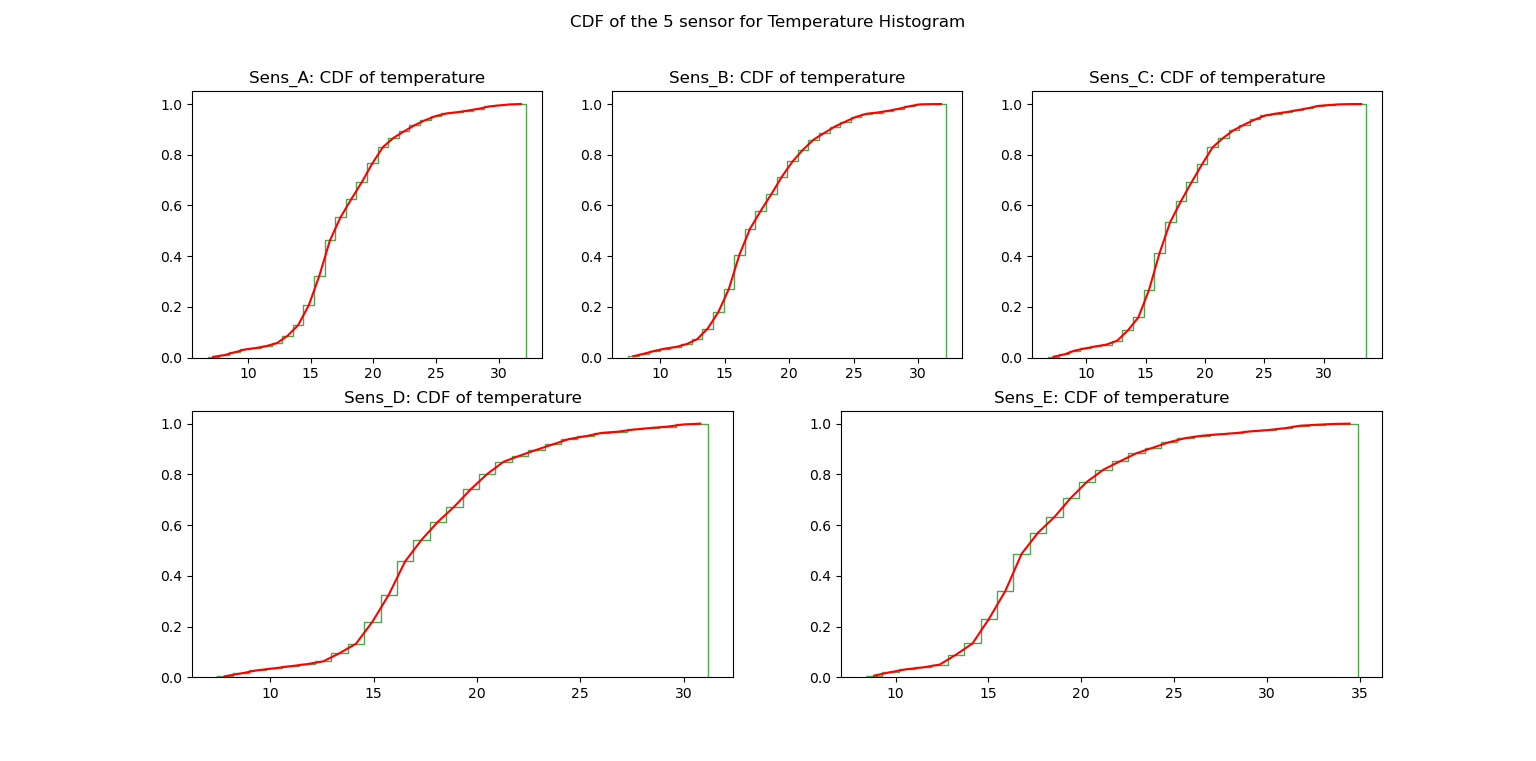
\includegraphics[width=\textwidth]{Graphs/CDF_of_the_5_sensor_-_Temperature_Histogram.png}
\caption{\it'CDF of the 5 sensor for Temperature Histograms'}
\end{figure}




Comparing the 3 distribution we can immediately figure out that there are major 
differences between each other as they use different methods. However, when comparing between sensors for each distribution the pattern remains basically the same. As for their tails, they seem to be right skewed.




\subsection{\it For the Wind Speed values, plot the pdf and the kernel density estimation. Comment the differences.}




For 2.2, the code outputs 5 plots of the PDF and KDE 
of the variable Wind Speed for each of the sensors. The figure(Figure 8) is a 
comparison between the PDF and the KDE of the above variable.



\begin{figure}[H]
\centering
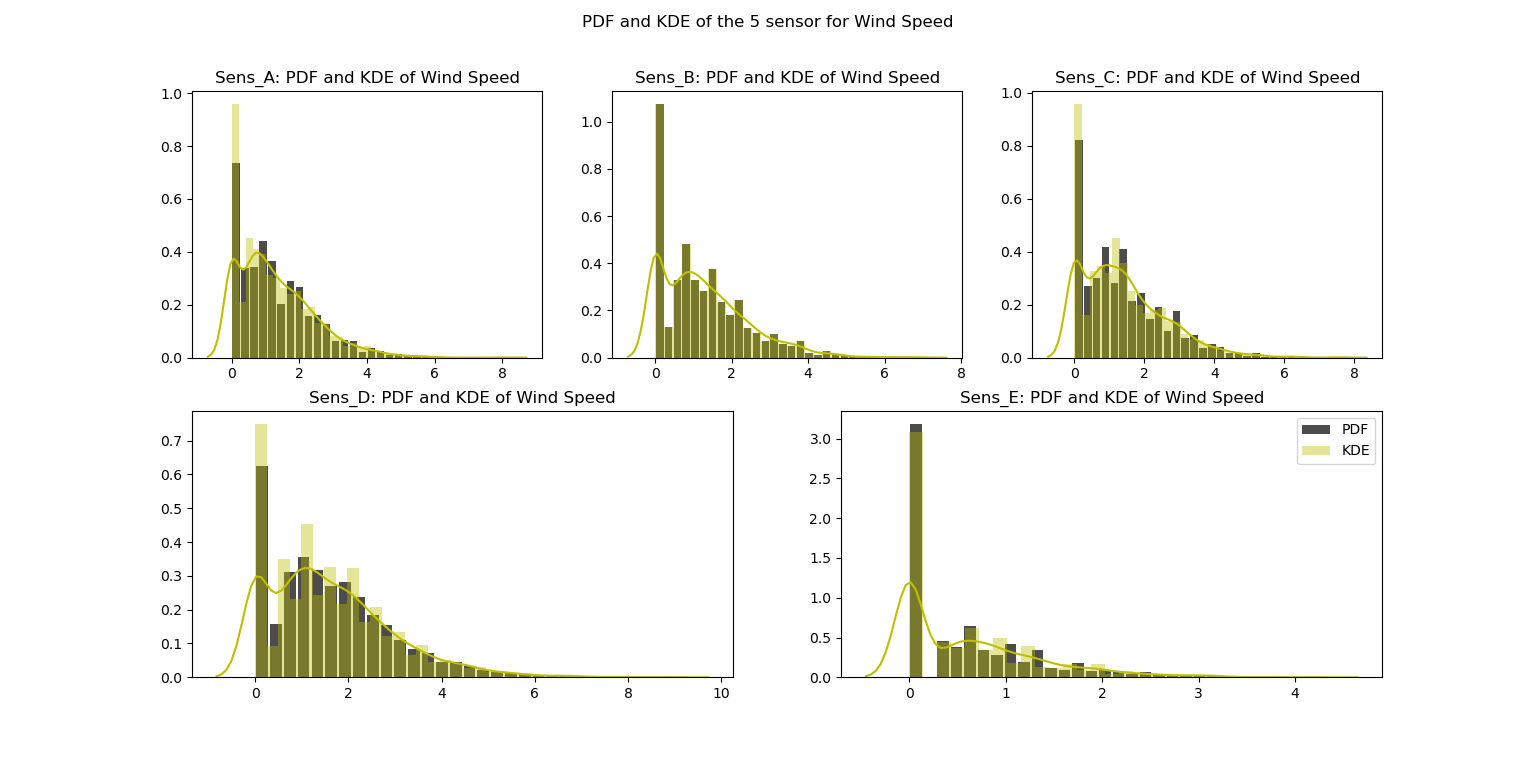
\includegraphics[width=\textwidth]{Graphs/PDF_and_KDE_of_the_5_sensor_-_Wind_Speed.png}
\caption{\it'PDF and KDE of the 5 sensor for Wind Speed'}
\end{figure}




As it is expected the KDE resembles the respective PDF as it smooths it out 




\section{\it After lesson A3:}
\subsection{\it Compute the correlations between all the sensors for the variables: Temperature, Wet Bulb Globe Temperature (WBGT), Crosswind Speed. Perform correlation between sensors with the same variable, not between two different variables; for example, correlate Temperature time series between sensor A and B. Use Pearson’s and Spearman’s rank coefficients. Make a scatter plot with both coefficients with the 3 variables.}




For 3.1, the codes computes Pearson’s and Spearman’s 
coefficients between all the of the 5 sensors for the variables Temperature, 
Wet Bulb Globe Temperature (WBGT), Crosswind Speed. The figure(Figure 9) illustrates the above mentions with 6 scatter plots 
(Pearson and Spearman for each variable). The sensor pairs are 10 in total (disregarding the symmetry).



\begin{figure}[H]
\centering
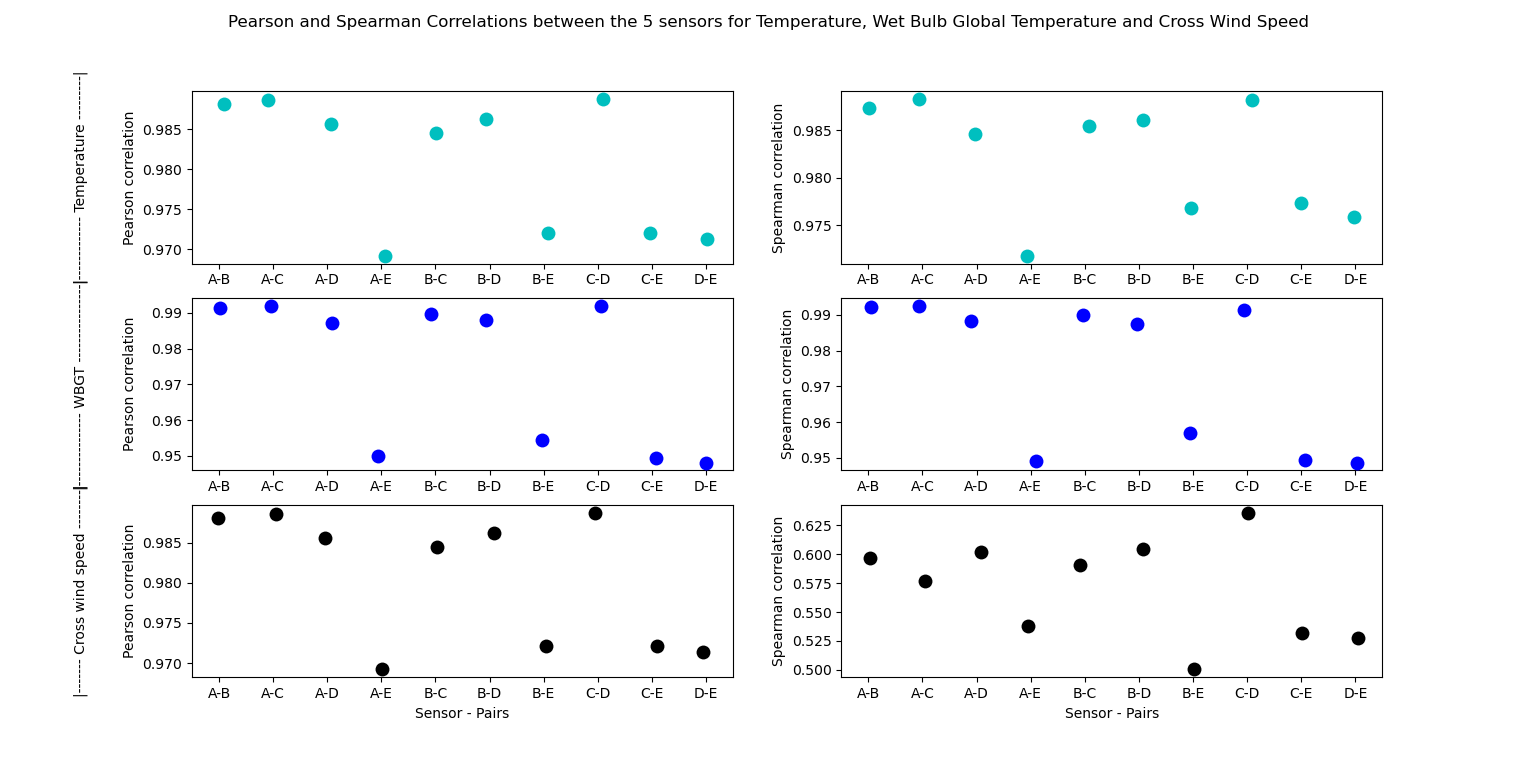
\includegraphics[width=\textwidth]{Graphs/Pearson-Spearman_5_sensors_Temp,_WBGT,CrWinSpeed.png}
\caption{\it'Pearson and Spearman Correlations between the 5 sensors for Temperature, Wet Bulb Global Temperature and Cross Wind Speed'}
\end{figure}




\subsection{\it What can you say about the sensors’ correlations?}





For 3.2, almost all of the correlations of the 
sensors tend to follow the same patterns. Overall, is seems that sensor E 
is considerably distant (in term of correlation) from the other sensors. In 
detail, sensor pairs A-B, A-C, A-D, B-C, B-D and C-D show that relate the highest, 
ranging from 98.4 to almost 100 percent. While sensor pairs A-E, B-E, C-E and 
D-E seem to fall behind by 1-3\%. The above correspond to all of the 3 variables for both correlation methods. 
However, for the variable Cross Wind Speed, Spearman’s method reveals an outlier in the overall correlation 
of the sensors for this variable. The pattern stays somewhat the same as the others, but with much lower overall correlation (from just 50 to 65\%). 




\subsection{\it If we told you that that the sensors are located as follows, hypothesize which location would you assign to each sensor and reason your hypothesis using the correlations.}




For 3.3, using the correlation of the sensors in combination with the proximity of the different sensors on the picture, we can guess their exact positions as below(Figure 10). 
The discrepancies in coefficients were such that the relative positions cannot 
be estimated with high certainty.



\begin{figure}[H]
\centering
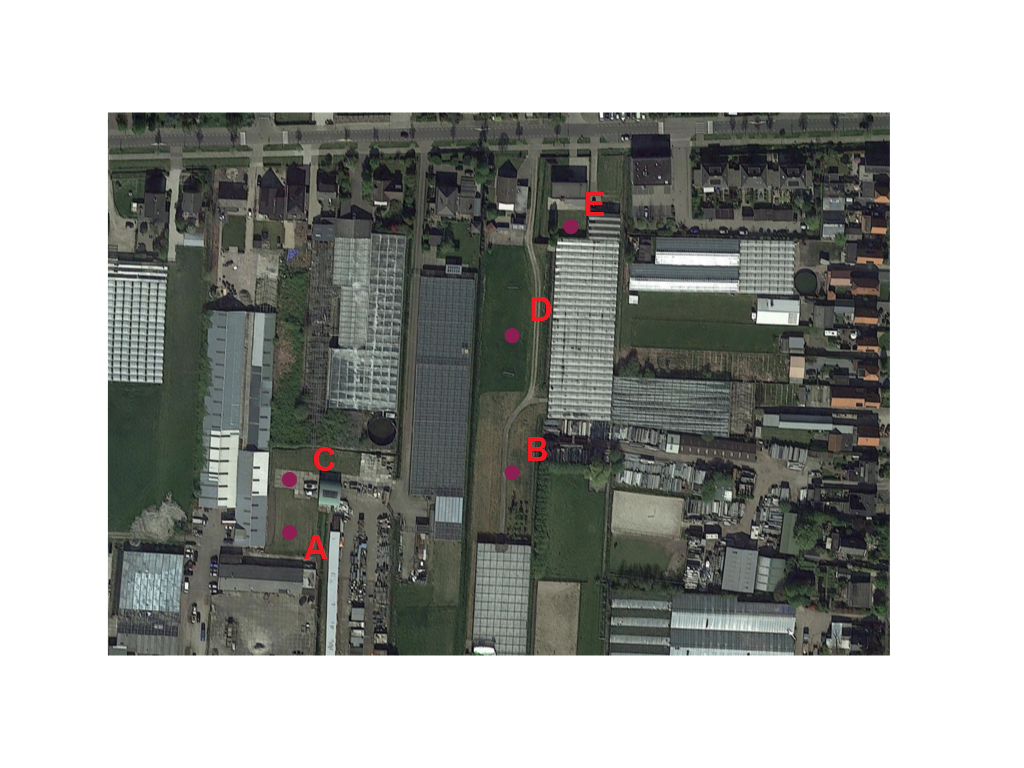
\includegraphics[width=\textwidth]{Graphs/SensorsSketch.png}
\caption{\it'Possible Sensor Positions'}
\end{figure}




\section{\it After lesson A4:}
\subsection{\it Plot the CDF for all the sensors and for variables Temperature and Wind Speed, then compute the 95\% confidence intervals for variables Temperature and Wind Speed for all the sensors and save them in a table (txt or csv form).}




For 4.1, the code creates the file confidence.txt where the 95\% 
confidence intervals for variables Temperature and Wind Speed 
for all the sensors are stored. Additionally, it shows a 
figure(Figure 11) of 10 plots for the CDFs (stepped histogram) of Temperature and Wind Speed for all the sensors.



\begin{figure}[H]
\centering
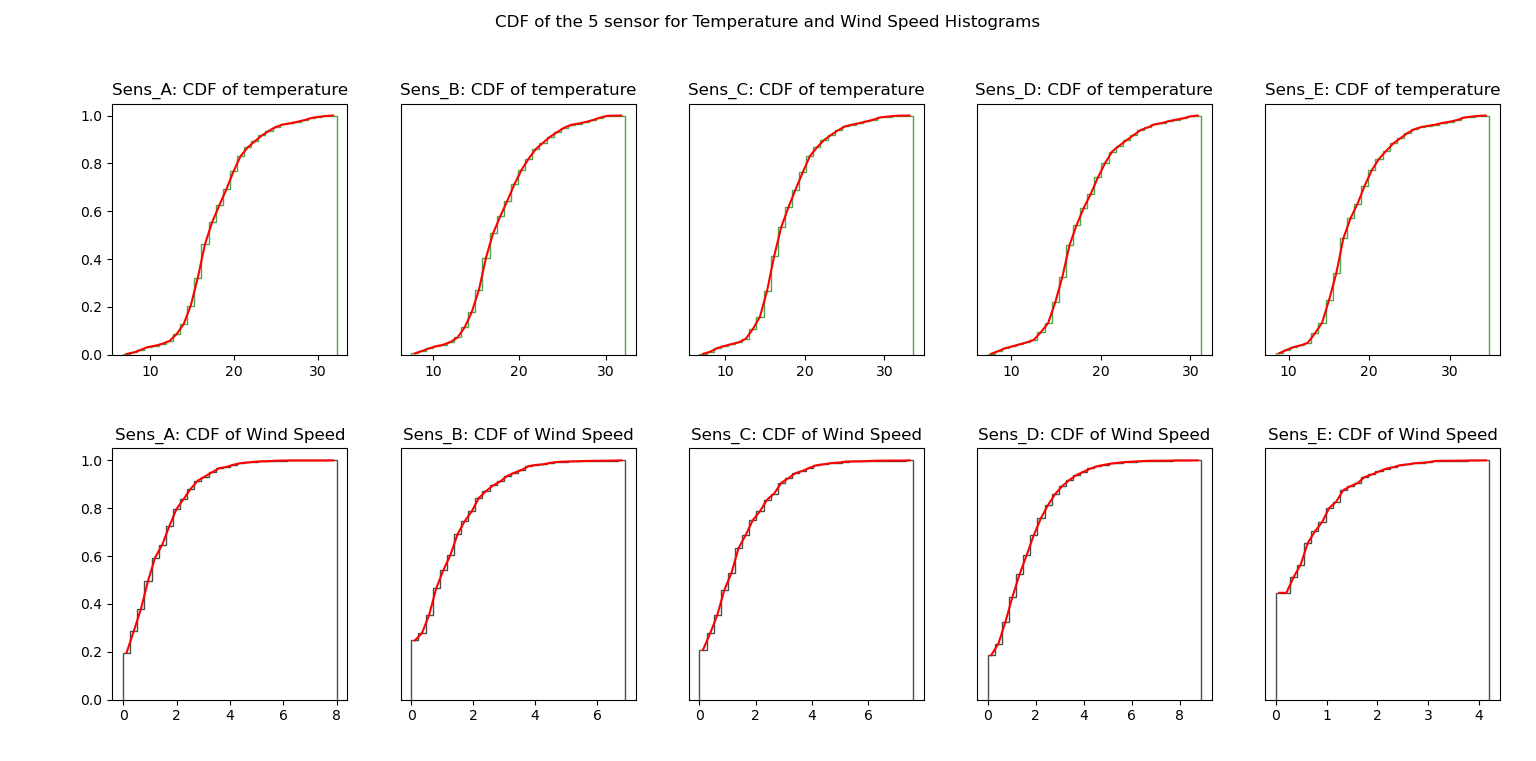
\includegraphics[width=\textwidth]{Graphs/CDF_of_the_5_sensor_-_Temperature,_Wind_Speed.png}
\caption{\it'CDF of the 5 sensor for Temperature and Wind Speed Histograms'}
\end{figure}



\begin{figure}[H]
    \centering
    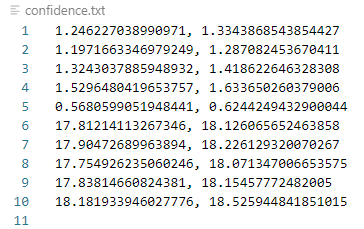
\includegraphics[width=0.5\textwidth]{Graphs/Confidence_95perc_Temp_WS.PNG}
    \caption{\it'95\% confidence intervals for Wind Speed(lines 1-5) and Temperature(lines 6-10) of all the sensors'}
    \end{figure}




\subsection{\it Test the hypothesis: the time series for Temperature and Wind Speed are the same for sensors}




\begin{itemize}
\item {1) E, D;}
\item {2) D, C;}
\item {3) C, B;}
\item {4) B, A;}
\end{itemize}




For 4.2, to test the hypothesis, the code computes with “ttest” the p-values of
the sensor pairs E-D, D-C, C-B, B-A (Figure 13). 




\subsection{\it What could you conclude from the p-values?}



\begin{figure}[H]
\centering
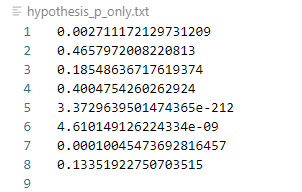
\includegraphics[width=0.5\textwidth]{Graphs/Pvalues_95pr_ttest_TEMP_WS.PNG}
\caption{\it'p-values from 't-test' for Temperature(lines 1-4) and Wind Speed(lines 5-8)'}
\end{figure}




Judging from the p-values, the conclusion for the temperature is:

\begin{itemize}

\item{E-D is statistically significant, null hypothesis rejected}


\item{D-C is statistically insignificant, null hypothesis accepted}


\item{C-B is statistically insignificant, null hypothesis accepted}


\item{B-A is statistically insignificant, null hypothesis accepted}

\end{itemize}

The conclusion for Wind Speed is:

\begin{itemize}

\item{E-D is statistically significant, null hypothesis rejected}


\item{D-C is statistically significant, null hypothesis rejected}


\item{C-B is statistically significant, null hypothesis rejected}


\item{B-A is statistically insignificant, null hypothesis accepted}

\end{itemize}

The condition that was used to test the hypothesis was:


p-value<0.05  ->  Reject


p-value>0.05  ->  Accept





\section{\bf Bonus Question:}


{\it Your “employer” wants to estimate the day of maximum and minimum potential energy 
consumption due to air conditioning usage. To hypothesize regarding those days, 
you are asked to identify the hottest and coolest day of the measurement time series provided. 
How would you do that? Reason and program the python routine that would allow you to identify those days.}




The measurements are taken every 20 minutes for every day of 24 hours (72 measurements pre day). 
So, the first step is to group the measurements for each day. To do this, the code selects all the values
of temperature that correspond to each different day, computes the mean of these values and matches them
inside a data-frame. After obtaining the mean temperatures for each day, the code finds the days where the maximum and minimum 
temperatures occurred (Table 1).




\begin{table}[H]
\begin{center}
\begin{tabular}[\textwidth]{|l|r|r|} \hline 
\centering
    Sensors     & Min           & Max           \\\hline
    Sensor A    & 10-06-2020    & 26-06-2020    \\\hline
    Sensor B    & 10-06-2020    & 26-06-2020    \\\hline
    Sensor C    & 10-06-2020    & 26-06-2020    \\\hline
    Sensor D    & 10-06-2020    & 26-06-2020    \\\hline
    Sensor E    & 08-07-2020    & 25-06-2020    \\\hline
\end{tabular}
\caption{'Days that maximum and minimum temperature measurements occure for each of the 5 sensors'}
\end{center}
\end{table}

From the table we can observe a major disparity for sensor E, getting the minimum temperature in a completely different day than the others.
It gets the maximum temperature a day before than the other sensors. It is an observation that was already identified from the graphs of this report. 
That said, the rest of the sensors agree on their values and as such we could hypothesize that the day with the least energy consumption for air-conditioning 
is the 10th of June 2020 and the day with the highest consumption, the 26th of June 2020.


The calculations were made with the assumption that
the term "Day" relates to a 24 hour day. In the occasion that the term "Day" corresponds to specific hours with sufficient sunlight, then at the first step we would have to
define these hours and grab their respective measurements to calculate the mean of the day. This depends completely on the employer's needs for air-conditioning.


\bibliographystyle{plain}
\bibliography{reference}

\end{document}
